\documentclass[a4paper,11pt, twoside]{book}

\usepackage[italian]{babel}
\usepackage[utf8x]{inputenc}
\usepackage{graphicx}
\usepackage{float}
\usepackage{url}
\usepackage[writefile]{listings}
\usepackage[Sonny]{fncychap}
\usepackage{fancyhdr}
\usepackage{supertabular}
\usepackage{longtable}
\usepackage[table]{xcolor}
\usepackage{array}
\usepackage{multirow}

\usepackage[italian]{babel}
\usepackage[utf8x]{inputenc}
\usepackage{graphicx}
\usepackage{float}

\usepackage{url}
\usepackage[writefile]{listings}
\usepackage{supertabular}
\usepackage{longtable}
\usepackage{booktabs}
\usepackage[table]{xcolor}


\usepackage{amssymb,amsmath}

\pagestyle{fancy}

%Impostazione capitoletti pagina
%\renewcommand{\chaptermark}[1]%
%{\markboth{\MakeUppercase{Capitolo \thechapter:\ #1}}{}}
%\renewcommand{\sectionmark}[1]%
%{\markright{\MakeUppercase{Sezione \thesection:\ #1}}}

%Impostazione linee di inizio e fine pagina
\renewcommand{\headrulewidth}{0.5pt}
\renewcommand{\footrulewidth}{0.2pt}

\newcommand{\helv}{%
\fontfamily{phv}\fontseries{b}\fontsize{9}{11}\selectfont}

\fancyhf{}
\fancyhead[LE,RO]{\helv \thepage}
\fancyhead[LO]{\helv \rightmark}
\fancyhead[RE]{\helv \leftmark}
\clearpage{\pagestyle{empty}\cleardoublepage}

\lstnewenvironment{xml}{\lstset{basicstyle=\footnotesize, frame=trbl, breaklines=true}}{} 
\begin{document}

  %Inizio Titolo
  \thispagestyle{empty}
    
  \begin{flushright}
    {Università degli Studi di Padova}\linebreak[1]
    \textbf{Corso di Laurea \linebreak Magistrale in Informatica} \linebreak \linebreak \linebreak \linebreak
  \end{flushright}
  
  \begin{center}
    {\texttt{Relazione del progetto per il corso di Sistemi Concorrenti e Distribuiti \linebreak \linebreak \linebreak \linebreak \linebreak}}
  \end{center}
  
  \begin{center}
    \texttt{\huge{\textbf{Simulatore concorrente e distribuito di una competizione di formula 1}}} \linebreak \linebreak \linebreak \linebreak \linebreak \linebreak \linebreak \linebreak \linebreak
  \end{center}
  
  
  \begin{flushleft}
    Studente: Cacco Federico\\Matricola: 624686\\Data: 16 giugno 2012
  \end{flushleft}

  \newpage
  \pagenumbering{Roman}
  \setcounter{page}{1}
  %Fine titolo

  \tableofcontents
  \newpage
  
  \chapter{Introduzione}
    \setcounter{page}{1}
    \pagenumbering{arabic}
    
    \section{Scopo del progetto}
      Il progetto didattico per il corso di Sistemi Concorrenti e Distribuiti consiste nell'analisi e la risoluzione 
      delle problematiche di progettazione di un simulatore concorrente e distribuito 
      di una competizione paragonabile ad una gara Formula 1.
      
      Ci sono vari aspetti di cui bisogna tener conto nella progettazione, come ad esempio la gestione
      dei sorpassi tra piloti e le politiche di utilizzo dei box.
      
      Addizionalmente ci sono tutta ua serie di parametri che possono influenzare le prestazioni di un concorrente,
      come ad esempio le condizioni meteo, le abilità dei piloti e le caretteristiche delle vetture

      Il sistema da simulare dovrà prevedere:
      \begin{itemize}
	\item Un circuito, possibilmente selezionabile in fase di configurazione, dotato almeno della pista e della corsia di 
	  rifornimento.
	  Entrambe dovranno essere soggette a regole congruenti di accesso, condivisione, 
	  tempo di percorrenza, condizioni atmosferiche, ecc.
	\item Un insieme configurabile di concorrenti, ciascuno con caratteristiche specifiche di prestazione, risorse, 
	  strategia di gara, ecc.
	\item Un sistema di controllo capace di riportare costantemente, consistentemente e separatamente, 
	  lo stato della competizione, le migliori prestazioni (sul giro, per sezione di circuito) e anche la 
	  situazione di ciascun concorrente rispetto a specifici parametri tecnici
	\item Una particolare competizione, con specifica configurabile della durata e controllo di terminazione 
	  dei concorrenti a fine gara.
      \end{itemize}
    
    \section{Struttura del documento}
      ******** DO-TO ********
  
  \chapter{Analisi dei requisiti}
    I requisiti funzionali obbligatori del progetto sono elencati nella tabella \ref{tbl:RequisitiFunzionaliObbligatori}
    
    \begin{longtable}{|p{2cm}|p{8cm}|}
      \toprule
	\bfseries{CODICE} & \bfseries{DESCRIZIONE} \\\hline
      \endfirsthead
      RFOBB-01 & Presenza di un circuito nella competizione \\\hline
      RFOBB-02 & Presenza di piloti nella competizione \\\hline 
      RFOBB-03 & Presenza di un sistema di controllo della competizione \\\hline
      RFOBB-04 & Il circuito deve essere dotato di una pista e della corsia di rifornimento \\\hline
      RFOBB-05 & La pista deve essere soggetta a regole congruenti di accesso \\\hline
      RFOBB-06 & La corsia dei box deve essere soggetta a regole congruenti di accesso \\\hline
      RFOBB-07 & La pista e la corsia box devono essere condivisibili tra i piloti \\\hline
      RFOBB-08 & La pista e la corsia box devono avere tempi di percorrenza verosimili \\\hline
      RFOBB-09 & La pista e la corsia box devono essere soggette a condizioni atmosferiche \\\hline
      RFOBB-10 & I concorrenti devono possedere personali caratteristiche di prestazione  \\\hline
      RFOBB-11 & I concorrenti devono possedere una strategia di gara  \\\hline
      RFOBB-12 & I concorrenti devono possedere una vettura con specifiche caratteristiche prestazionali  \\\hline
      RFOBB-13 & Il sistema di controllo deve riportare lo stato della competizione  \\\hline
      RFOBB-14 & Il sistema di controllo deve riportare le prestazioni e o stato dei piloti  \\\hline
      RFOBB-15 & Il sistema di controllo deve tener traccia delle migliori prestazioni  \\\hline
      RFOBB-16 & Durata e condizione meteo della gara devono essere configurabili  \\\hline
      RFOBB-17 & Presenza di un controllo di terminazione dei concorrenti a fine gara  \\\hline
      \caption{Requisiti funzionali obbligatori}
      \label{tbl:RequisitiFunzionaliObbligatori}
    \end{longtable}

    I requisiti funzionali opzionali del progetto sono invece elencati nella tabella \ref{tbl:RequisitiFunzionaliOpzionali}
    
    \begin{longtable}{|p{2cm}|p{8cm}|}
      \toprule
	\bfseries{CODICE} & \bfseries{DESCRIZIONE} \\\hline
      \endfirsthead
      RFOPZ-01 & Il circuito può essere scelto in fase di configurazione \\\cline{1-2}
      RFOPZ-02 & I piloti devono poter essere configurabili \\\cline{1-2}
      \caption{Requisiti funzionali opzionali}
      \label{tbl:RequisitiFunzionaliOpzionali}
    \end{longtable}
    
  
  \chapter{Progettazione}
    \section{Entità coinvolte}
      Durante la fase di progettazione sono state individuate le seguenti entità costitutive:
      
      \begin{itemize}
        
	\item Gara 
	\item Concorrenti
	\item StartUp
	\item Sender
	\item Monitor

      \end{itemize}
      
      
      Concorrenti e Gara hanno vari parametei di configurazione che vengono impostati prima 
      dell'esecuzione del programma
      
      Di seguito verranno descritte in modo più approfondito per chiarire il loro compito all'interno del
      programma.
      
    \section{Gara}
      L'entità Gara rappresenta la competizione vera e propria nella quale si sfideranno i vari
      concorreti. Essa è descitta dale seguenti proprietà:
      
      \begin{itemize}
	\item Circuito
	\item Numero di giri
	\item Meteo
      \end{itemize}
	
      \subsubsection{Meteo}
        Può essere ascutto o bagnato, e rappresenta la condizione climatica al momento della gara.
        Nel caso in cui esso sia impostato su bagnato si avranno dei peggioramenti nei tempi con cui ogni pilota
	completerà i giri della pista, simulando quindi un asfalta bagnato e con meno aderenza
	
      \subsubsection{Circuito}
        Rapprensenta il tracciato su cui si svolge la competizione, contiene le informaziono ad esso relativo come
	ad esempio il nome e la sua conformazione
	
        Come detto rapresenta il tracciato su cui si svolge la competizione. Dato che in un reale circutio di formula uno
	si possono distinguere ratti di pista con carateriscitche diverse come ad esempio curve e rettiliei o anche
	tratti che consentono o meno ai vari piloti i sorpassarsi.
	
	Questi aspetti sono stati presi in considerazion anche nella realizzazione del progetto, per cui si è deciso
	di suddividere il tracciato in vari segmenti, ovvero tratti di pista con caratterisciche uguali
	
	Un tracciato contiene quiandi le seguenti proprietà:
	
	\begin{itemize}
	  \item Nome del circuito
	  \item Numero di segmenti
	  \item Lista dei segmenti
	  \item Griglia di partenza
	  \item Lunghezza del giro
	\end{itemize}
	
	
	I segmenti rappresentano i tratti di poista che un pilota dovra percorrere per completare un giro.
	Ogni segmento contiene la descizione del ratto di psta che rappresenta e si occupa di
	fornire ai piloti il tempo necessario per il suo atraversamento, gestendo anche gli eventuali sorpassi 
	(questi aspetti saranno chiariti poi nella sezione METTERE RIFERIMENTO) 
	
	La griglia di partenza è il luogo dove i piloti si scherano in attesa di partire, anche questo aspetto
	verrà chiarito nella sezione METTERE RIFERIMENTO
	
	
	La griglia di partenza e i segmenti sono le entità che gestico l'aspetto concorrente del progetto,
	questi aspetti verranno descritti nella sezione 
	
        
	
	Ogni segmento contiene le seguenti proprietà
	\begin{itemize}
	  \item Codice univoco
	  \item Tipologia
	  \item Lunghezza
	  \item Velocità massima
	  \item Numero di cosie
	  \item Presenza fotocellula
	\end{itemize}
	
	
	
	
	
	
	
	
        
	nel quale si svolge la gara, dato che non deve 
	eseguire alcuna azione si
	tratta di una entità passiva che ha lo solo scopo di accogliere i piloti impegnati ad affrontare la
	competizione.
	Dovrà comunque regolamentare la loro attività garantendo che vengano rispettate delle regole di accesso congrue
	ad una ipotetica competizione reale. 
	Le caratteristiche e le regole che il circuito dovrà fornire saranno le seguenti:
	
	\begin{itemize}
	  \item Dovrà essere specificata una lunghezza del circuito
	  \item Il circuito deve avere una larghezza variabile durante la sua percorrenza, non in tutti i tratti sarà
		ad esempio possibile eseguire un sorpasso per via dello spazio limitato
	  \item Nel circuito dovranno essere presenti sia tratti curvi che rettilinei, che avranno quindi diverse velocità
		di percorrenza
	  \item Dovranno esserci dei punti per il rilevamento delle prestazioni
	  \item Dovrà essere presente una corsia per i box, con relative regole di accesso
	  \item Tutte queste opzioni dovranno poter essere configurate mediante file di configurazione
	\end{itemize}
	
	Questa risorsa sarà condivisa da più piloti allo stesso tempo, sarà quindi necessario gestire
	tutte le problematiche di concorrenza derivate.
	
	METTERE DESCRIZONE TIPI SEGMENTO
	
	
	
	
      
    \section{Piloti}
      I piloti sono le entità che dovranno gareggiare nella competizione atraversando il circuito.
      Lo scopo di ognuno di essi è quello di percorrer tutti i giri prefisti nella gara nel mimor tempo possibile,
      il tutto in modo coerente con le caratteristiche del circuito.
      
      Dato che nella realtà ogni pilota ha le proprie abilità (come ad esempio la prontezza di riflessi
      o la capacità di valutare i punti esatti in cui effettuare le staccate) \footnote{Con il termine staccata si indica 
      la fase in cui un pilota dopo un tratto rettilineo frena bruscamente per iniziare l'inserimento in curva},
      anche in questo caso ad ogni pilota dovranno essere associate delle caratteristiche, chiamate skill, che possano
      modellarne il comportamento in pista. Le skill che ogni pilota poeediede sono:
      
      \begin{itemize}
	\item Numero del pilota
	\item Nome del pilota
	\item Skill di accelerazione
	\item Skill di decellerazione
      \end{itemize}
      
      La skill di ascelerazione e la skill di decellarazione indicano rispettivamente la capacità del pilota di frenare 
      il più tardi possibile prima di un inserimento in curva e la capicità del pilota di iniziare l'accelerazione 
      il più presto possibile. Bassi valori in queste skill implicheranno che il pilota iniziarà a frenare troppo presto 
      e ad eccelerare troppo tardi rispetto all'istante ottimale, peggiorando così le sue prestazioni nel giro di pista.
      
      Ad ogni pilota viene poi associata una vettura, anch'essa caratterizzata da delle skill che ne influenzeranno
      le prestazioni in pista. Esse sono:
      
      \begin{itemize}
	\item Costruttore
	\item Coefficente di accelerazione
	\item Coefficente di decellazione
	\item Velocità massima
	\item Tenuta di strada
	\item Consumo degli pneumatici
      \end{itemize}
      
      Il coefficente di accelerazione e di decellazione indicano le prestazioni di accelerazione e frenata della vettura, 
      vetture con alti coefficenti avrano quindi migliori capacità di cccelerazione e decellerazione
      che comporterano prestazioni migliori
      
      La tenuta di strada viene invece usata per calcolrae i tempi di perorrenza nelle curve e quanto peggiorano 
      le prestazioni in caso di pista bagnata
      
      Il consumo degli peumatici invece stabilice in quanti giri essi degradano e hanno bisogno di essere sostiuiti
      ai box. Vetture con un basso degrado degli pneumatici potranno compiere più giri senza doversi vermare ai box
      
      Ogni pilota inoltre possiede un propria strategia, che rappresenta l'elenco dei giri in cui fermarsi per effettuare il
      calmbio gomme
      
      Inoltre piloti con un basso consumo di caburante potranno completare la gara immagazinando alla partenza un minor
      quantitativo d'esso, rendendo così la vettura più leggera e performante
      
      \subsection{Fasi della gara}
	\subsubsection{Partenza}
	  Questa è la prima fase della gara, semplicemente una volta che il pilota è stato creato
	  viene posizionato nella griglia di partenza nell'attesa di iniziare la gara.
	  
	  Una volta che tutti i piloti saranno schierati la gara potrà partire e i piloti inizieranno a gareggiare
	  
	\subsubsection{Attraversamento dei segmenti}
	  In questa fase i piloti attraversano i vari segmenti del tracciato nel tantativo di completare tutti i giri
	  il primapossibile.
	  
	  L'attraveramento di un segmento si svolge in modo analogo sia che il tratto di pista sia
	  di accelerazione, di frenata oa veocità costante (curva), cambia solo il modo co cui esso viene 
	  determinato il tempo di atraversamento
	  
	  \paragraph{Tratto di acelerazione\\}
	    Nel caso in cui il pilota sia impegnato in un tratto di accelerazione, percorrenzacalcolare io tempo del
	    del suo atraversamento vengono seguiti questi passiva
	    
	    \begin{enumerate}
	      \item In base alle caratterisctiche del pilota viene calcolato lo spazio di ritardo con cui il
		    pilota inizierà l'acelerazione. Tale spazio potrà essere al massimo il 10$\%$ della lunghezza del segmento
	      \item Viene quindi calcolato lo spazio effettivo di acelerazione $SA_{eff}$, che sarà quindi tanto maggiore quanto
		    il pilota sarà abile nell'accelerare il prima possibile
	      \item In base dello spazio di acelerazione effettivo viene calolata la velocità massima che il pilotà avrà alla fine del 
		    tratto di acelerazione,
		    tale velocità sarà ridotta al massimo del 10$\%$ sulla base delle prestazioni in acelerazione della vettura,
		    e non sarà comunque superiore alla velocità massima della vettura
	      \item Sulla base della velocità di entrata del segmento e di quella di uscita si calcola il tempo di attraversamento
	      \item Si calcolano poi delle penalità che verranno aggiunte a tale tempo, che sono:
		    \begin{itemize}
		      \item Condizioni meteo e tenuta di strada
		      \item Stato degli pneumatici
		      \item Peso della benzina nella vettura
		    \end{itemize}
		    Tali penalità vengono poi sommate al tempo di attraversamento
	      \item A questo punto il pilota chede l'accesso alla risorsa protetta del segmento
		    comunicando i tempo atteso per l'attraversamento. La risporsa risponde comunicando il tempo
		    efettivo di atraversamento sulla base della presenza o meno di altri piloti.
	      
	      \item a tale tempo vengono aggiunte delle penalita (ciascuna non superiore al 10\% del tempo di attraversamento)
	      \item Viene calcolato un empo ideale Ta di attraversamento in base alla funzione di simulaziome dell'accelerazione
	      \item Si aggiunge una penalità massima del 10\% in base  
	    \end{enumerate}
	    
	  \paragraph{Tratto di decellerazione}
	    Nel caso in cui il pilota sia impegnato in un tratto di decellerazione, percorrenzacalcolare io tempo del
	    del suo atraversamento vengono seguiti questi passiva
	    
	    \begin{enumerate}
	      \item Viene calcolato lo spazio di frenata in base al punteggio di frenata dell'auto
	      \item In base alle caratterisctiche del pilota viene calcolato lo spazio di anticipo con cui il
		    pilota inizierà la decelerazione. Tale spazio potrà essere al massimo il 10\% della lunghezza del segmento
		    Maggiore è questo spazio maggiore sarà l'anticipo della frenata, fatto che causerà una dimnuzione delle prestazioni.
		    
	      \item Viene quindi calcolato lo spazio effettivo di frenata $SA_{eff}$, che sarà quindi tanto maggiore quanto
		    il pilota sarà abile nell'accelerare il prima possibile
	      \item In base dello spazio di acelerazione effettivo viene calolata la velocità massima che il pilotà avrà alla fine del 
		    tratto di acelerazione,
		    tale velocità sarà ridotta al massimo del 10\% sulla base delle prestazioni in acelerazione della vettura,
		    e non sarà comunque superiore alla velocità massima della vettura
	      \item Sulla base della velocità di entrata del segmento e di quella di uscita si calcola il tempo di attraversamento
	      \item Si calcolano poi delle penalità che verranno aggiunte a tale tempo, che sono:
		    \begin{itemize}
		      \item Condizioni meteo e tenuta di strada
		      \item Stato degli pneumatici
		      \item Peso della benzina nella vettura
		    \end{itemize}
		    Tali penalità vengono poi sommate al tempo di attraversamento
	      \item A questo punto il pilota chede l'accesso alla risorsa protetta del segmento
		    comunicando i tempo atteso per l'attraversamento. La risporsa risponde comunicando il tempo
		    efettivo di atraversamento sulla base della presenza o meno di altri piloti.
	      
	      \item a tale tempo vengono aggiunte delle penalita (ciascuna non superiore al 10\% del tempo di attraversamento)
	      \item Viene calcolato un empo ideale Ta di attraversamento in base alla funzione di simulaziome dell'accelerazione
	      \item Si aggiunge una penalità massima del 10\% in base  
	    \end{enumerate}

	    
	    
	  partenza 
	  atraversamento segmenti
	  eventuali soste
	  fine gara
      \subsection{Simulazione accelerazione}
	Dato che simulare la reale curva di accelerazione di una vettura di formula è una operazione complessa,
	è stato deciso di semplificare la sua rappresentazione.
	L'aspetto chiave da tenere in considerazione è il fatto che essa varia in funzione della velocità, più precisamente
	più bassa è la velocità e maggiore è l'accelerazione che si riesce ad impremere alla vettura
	
	I più, dato che tutto il sstema di riferimento è in base allo spazio percorso e non al tempo, la velocità
	viene calcolata in base alla distanz percorsa e non in base al tempo
	
	La funzione scelta per rappresentare la velocità in funzione della distanza percorsa è 
	dunque la seguente:
	
	$$METTERE FUNZIONE$$
	
	Nella figura \ref{fgr:GraficoVelocita} viene rappresentato il grafico della funzione usata per simulare il valore
	della velocità raggiunta in funzione della distanza percorsa.
	
	\begin{figure}[h]
	  \centering
	  \fbox{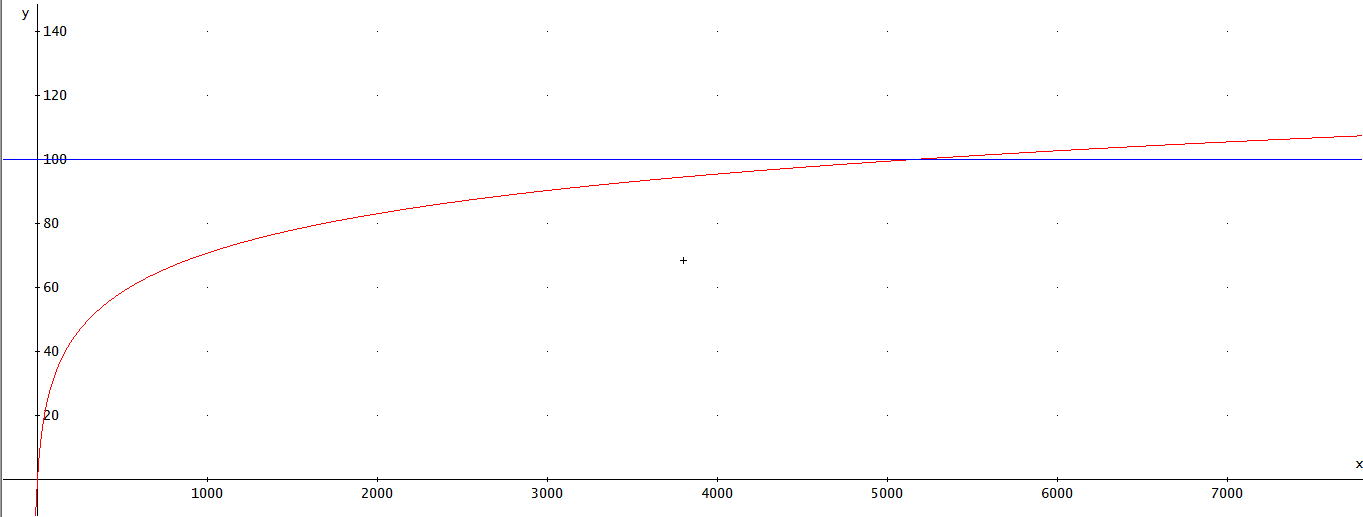
\includegraphics[width=120mm,bb=0 0 991 376]{./Immagini/GraficoVelocita.png}}
	  % GraficoVelocità.png: 1363x517 pixel, 99dpi, 34.97x13.26 cm, bb=0 0 991 376
	  \caption{Andamento della velocità in base alla dstanza percorsa di una vettura con velocità iniziale
		    pari a 0m/s}
	  \label{fgr:GraficoVelocita}
	\end{figure}
	
	Tale grafico presuppone che la vettura parta da una velocità iniziale di 0m/s, ma questo si verifica solo 
	alla partenza.
	Per calcolare la variazione di velocità della vettura in funzione della distanza pecorsa, nel caso in cui la vettura
	abbia una velocità iniziale v0 è sufficente traslare il grafico fino a intersecare tale valore di partenza con l'asse
	delle ordinate, come nell'esmpio in figura \ref{fgr:GraficoVelocitaTraslato}
	
	\begin{figure}[h]
	  \centering
	  \fbox{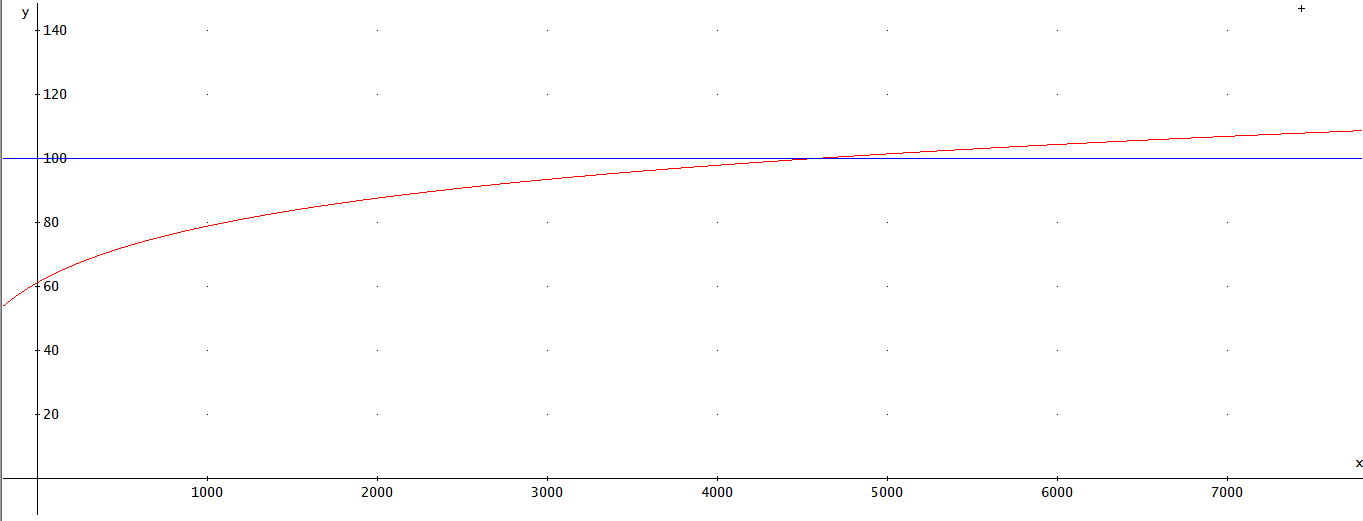
\includegraphics[width=120mm,bb=0 0 991 376]{./Immagini/GraficoVelocitaTraslato.png}}
	  % GraficoVelocità.png: 1363x517 pixel, 99dpi, 34.97x13.26 cm, bb=0 0 991 376
	  \caption{Andamento della velocità in funzione della distanza, assumento che la vettura abbia una
		    velocità iniziale di 60m/s}
	  \label{fgr:GraficoVelocitaTraslato}

	\end{figure}
	
	Il valore finale sarà poi ridimensionato in base alle caratterisitche della ettura
	Il valore finale della velocità non potrà comunque essere superiore a quello massimo raggiungibile dalla vettura

      \subsection{Simulazione decellerazione}
	La decellerazione risulta molto più semplice rispetto a quella dell'accelerazione i quanto
	si può approssimare il fatto che durante la frenata la forza inpressa dal freno sia costante
	
	La formula con la quale essa viene odellata è la seguente:
	
	$$METTERE FORMULA DECELLAZIONE$$
	
      \subsection{Simulazioe tratto a velocità costante}
      
      \subsection{Srategia}
      
	I piloti avranno poi una loro personale strategia di gara, questo consentirà loro di effettuare
	i sorpassi non solo durante la percorrenza del giro, ma anche raggiungendo un buon compromesso
	tra numero di soste ai box e prestazioni su pista. Infatti maggiori saranno le soste e migliori saranno le prestazioni
	sul giro, dato che il pilota avrà presumibilmente un minore quantitativo di benzina, e quindi un minor peso, nella vettura.
	Bisognerà fare comunque attenzione che la programmazione delle soste sia tale da consentire al pilota di concludere la gara,
	evitando che esso finisca l carburante prima del suo termine
      
      Le caratteristiche che dovranno avere i piloti saranno quindi:
	
	\begin{itemize}
	  \item Nome 
	  \item Numero
	  \item Skill misurante la capacità di eseguire il prima possibile le accelerazioni in uscita dalle curve
	  \item Skill misurante la capacità di ritardare il più possibile la staccata prima di un inserimento in curva 
		\footnote{La staccata dovrà essere comunque effettuata in modo tale da garantire la 
		corretta percorrenza della curva}
	  \item Un strategia di gara che regoli le soste ai box
	\end{itemize}
	
	
	Ad ogni pilota sarà poi assegnata una vettura, anche questa dotata di determinate caratteristiche che influenzeranno il suo
	comportamento in pista. Esse saranno:
	
	\begin{itemize}
	  \item Nome del costruttore
	  \item Forza frenante
	  \item Potenza di accelerazione
	  \item Tenuta in curva
	  \item Consumo per chilometro
	  \item Velocità massima
	  \item Livello attuale di carburante
	\end{itemize}
      
      

     
	
    \section{Sender}
      % \<TO DO\>
      Questa entità si occupa di inizializzare l'intera competizione e di avviare la gara.
      Contiene meteo, numero di giri, piloti.....
      
    \section{Monitor}
  
    \section{Concorrrenza}
      Gli aspett del progetto in cui entrano in giorcho problemi di natura concorrenziale sono 3:
      
      \begin{itemize}
        \item Schieramento nella griglia di partenza
	\item Attraversamento dei segmenti da parte dei piloti
      \end{itemize}
      
      \subsection{Schieramento nella griglia di partenza}
        La griglia di partenza è stata modellata come una risorsa protetta, in modo da potervi accodare i piloti
	fino nell'attesa della partenza.
	
	Questo è stato necessario in quanto la gara può partire solo una volta che tutti i piloti sono stati schierati,
	
	La risorsa protetta contiene 3 canali d'accesso:
	\begin{itemize}
	  \item Uno pubblico sempre aperto chiamato Place\_On\_Grid
	  \item Uno privato controllato da una guardia chiamato  Wait\_To\_Start
	  \item Uno pubblico controllato da guardia chiamato Wait\_To\_Pilots
	\end{itemize}
	
	Il protocollo d'accesso alla griglia di partenza è il seguente, e comprende 2 serie di eventi
	concorrenti:
	
	Thread di gestione della gara
	\begin{itemize}
	  \item Una volta che ha creato tutti i piloti chiede acesso al canale Wait\_To\_Pilots,
	        inizialmente con guardia chiusa
          \item Una volta che tutti i piloti sono shierati la guardia viene aperta e il controllore
	        si pone in attesa del segnale di inizio gara da parte dell'utente
	  \item Una volta ricevuto tale segnale viene aperta la guardia Wait\_To\_Start
	\end{itemize}
	
	Thead dei piloti:
	\begin{itemize}
	  \item Un pilota viene creato e chiede di schierarsi nella griglia di partenza tramite il canale Place\_On\_Grid
	  \item Il numero di piloti in griglia viene aumentato di uno
	  \item Il pilota viene riaccodati nel canale Wait\_To\_Start (inizialmente chiuso)
	  
	  \item Quando il numero dei piloti schierati è uguale al nunero di piloti che devono prendere parte alla gara
	        la guardia di Wait\_To\_Pilots viene aperta
          \item i piloti atendono ora l'apertura della guardia Wait\_To\_Start da parte del controllore
	\end{itemize}

	      
      \subsection{Acceso ai segmenti}
        L'accesso ai segmenti è la parte crucil della gara, in quanto tramite essi viene gestita
	tutta la dinamica della gara, ovvero tempi di percorrenza del circuito, sorpassi e accesso ai box
	
	Come detto un segmento è composto da una o più corsie gestite mediante una risorsa protetta per garantire
	l'accesso in mutua esclusione, queste consentono ai piloti di entrare nello stesso segmento 
	contemporaneamente e di effettuare sorpassi.
	Se un segmento è composto da una sola corsia i piloti dovranno necessariamente accodarsi in un'unica fila e attraversare
	il segme nto serza alcuna possibilità di effettuare sorpassi
	
	L'accesso viene modellato mediante una risorsa protetta associata a ciascun segmento, che contiene
	la rappresentazione delle sue corsie e il loro stato, overo per ogni corsia viene memoriazzato l'istante
	in cui l'ultimo pilota uscirà da essa
	
	La modalità d'accesso ai segmenti non varia in base alla sua tipologia, restando la medesima per ognuno d'essi.
	
	Per semplicità il protocollo d'accesso verrà spigato tramite un esempio. Supponiamo dunque che un pilota C
	voglia attraversare un generico segmento S composto da 2 corsie, esso effettuerà per prima cosa le seguenti operazioni:
	
	\begin{itemize}
	  \item Reperimento delle informazioni del segmento
	  \item Calcolo del tempo di attravesamento ideale $T_i$ in base al suo stato e alle caratteristiche del segmento
	  \item Accesso in utua esclusione alla risorsa protetta del segmento
	  \item Chiamata al metodo della risorsa protetta del segmento, che risponderà comunicando il reale tempo
	        di attravarsamento $T_r$ calcolato in base al suo stato
          \item Aggiornameto dello stato della risorsa protetta
          \item Rilascio della risorsa protetta
          \item Sospensione del pilota per un tempo $T_r$
	\end{itemize}
	
	$T_i$ non fa nessuna considerazione sugli aspetti relativi alla concorrenza, ma calcola il tempo
	assumendo che il segmento non sia accupato da nessuna vettura. Questo tempo serve alla risorsa protetta come
	base di partenza per calcolare $T_r$
	
	Il procedimento con cui viene calcoltato $T_r$ può essere spiegato mediante un esmpio,
	poi facilmemnte generalizzabile.
	
	Supponiamo quaindi che all'istante $T_0=0$ un pilota $P_c$ debba attraversare un segmento $S$ 
	con 2 corsie che si trovano nel seguente stato:
	
	\begin{itemize}
	 \item Corsia 1 occuopata da un pilota $P_a$ con istante d'uscita $T_{Pa}=16$
	 \item Corsia 1 occuopata da un pilota $P_b$ con istante d'uscita $T_{Pb}=8$
	\end{itemize}
	
	$T_{c1}$ e $T_{c2}$ sono gli istanti in cui l'ultimo pilota libera rispettivemente la corsia 1
	e la corsia 2, quiandi si avrà $T_{c1} = T_{Pa}$ e $T_{c2} = T_{Pb}$
	
	Uno schema dello stato del segmento è rappresentato nella figura \ref{fgr:AccessoSegmentiStatoInziale}
	
	\begin{figure}[h]
	  \centering
	  \fbox{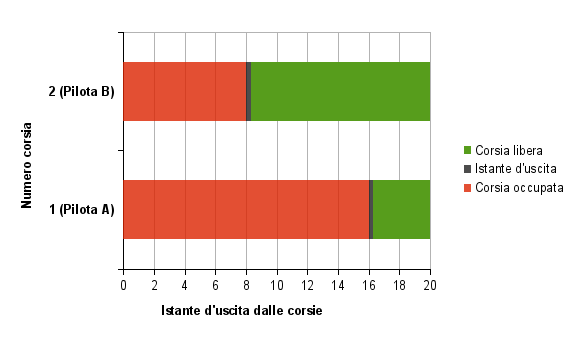
\includegraphics[width=110mm,bb=0 0 575 338]{./Immagini/AccessoSegmentiStatoInziale.png}}
	  % AccessoSegmentiStatoInziale.png: 575x338 pixel, 72dpi, 20.28x11.92 cm, bb=0 0 575 338
	  \caption{Stato del segmento S all'istante in cui il pilota C chiede l'accesso}
	  \label{fgr:AccessoSegmentiStatoInziale}
	\end{figure}
	
	Ora a seconda del valore di $T_i$ relativo al pilota A si possono ipotizzare tre possibili scenari, che sono
	
	\begin{itemize}
	 \item $T_i < T_a$
	 \item $T_a < T_i < T_b$
	 \item $T_i > T_b$
	\end{itemize}
	
	Occorre anche introdurre un tempo chiamato $T_{min}$, ovvero il distacco minimo che 2 vetture possono avere
	stando sulla stessa corsia senza sovvrapporsi
	Vediamo ora come si calcolerà il tempo d'uscita del pilota $P_c$ per ognuni di questi 3 casi.
	
	
	\subsubsection{Caso $T_i < T_a$}
	  In questo caso il pilota $P_c$ uscirebbe sia prima di $P_a$ che di $P_b$, questo tuttavia non è possibile in quanto
	  entrambe le corsie sono già occupate da piloti che la liberano dopo di lui in quanto $T_i < T_a < T_b$
	  
	  Il pilota $P_{c}$ verrà dunque inserito nella corsia con il tempo di uscita minore, ovvero $C_2$,
	  e quindi attraverserà il segmento $S$ usando la corsia $C_2$ in tempo $T-r = T{c1} + T_{min}$
	  usacendo subito dopo il pilota $P_2$. L'ordine d'uscita dal segmento sraà dunque $P_a -> P_c -> P_b$
	  ($P_c$ riesce a sorpassare $P_b$)
	  
	  Bisognerà poi aggiornare lo stato del segmento, ponendo l'aggiornamento dello stato del segmeneto ponendo
	  $T_{C1 = T_r}$ i quanto ora $P_c$ è l'ultimo pilota ad uscira dalla corsia $C_2$, uno schema del
	  nuovo stato del segmento è riportato nella figura \ref{fgr:AccessoSegmentiCaso1}
	  
	  \begin{figure}[h]
	    \centering
	    \fbox{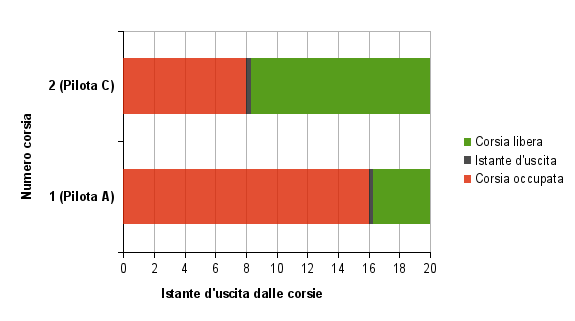
\includegraphics[width=110mm,bb=0 0 575 338]{./Immagini/AccessoSegmentiCaso1.png}}
	    % AccessoSegmentiStatoInziale.png: 575x338 pixel, 72dpi, 20.28x11.92 cm, bb=0 0 575 338
	    \caption{Caso 1: Stato del segmento S dopo che il pilota C ha effettuato l'accesso}
	    \label{fgr:AccessoSegmentiCaso1}
	  \end{figure}
	  
	\subsubsection{Caso $T_a < T_i < T_b$}
	  In questo caso il pilota $P_c$ uscirebbe dopo $P_a$  prima di $P_b$, questo è compatibile con 
	  lo stato del segmento in quando $P_c$ vede la corsia $C_1$ vitualmente libera in quanto
	  il pilota che la impegna esce in ogni caso prima di lui e non comporta nessun ostacolo alla sua percorrenza
	  
	  $P_c$ viene dunque inserito nella corsia con il tempo d'uscita minore, ovvero $C_2$ e dato che
	  $T-i < T_{C2}$ potrà attraversare il segmento in un tempo $T_r = T_i$. 
	  Nello stato della risorsa protetta del segmento verrà posto $TC_2 = T_r$, mentre $T_C1$ resterà invariato.
	  L'ordine d'uscita sal segmento sarà poi $P_a -> P_c -> P_b$, e il pilota $P_c$ avrà effettivamente 
	  superato $P_b$ come previsto.
	  
	  Uno schema del nuovo stato della risorsa protetta relativa al segmento $S$ è illustrato nella figura 
	  \ref{fgr:AccessoSegmentiCaso2}

	  \begin{figure}[h]
	    \centering
	    \fbox{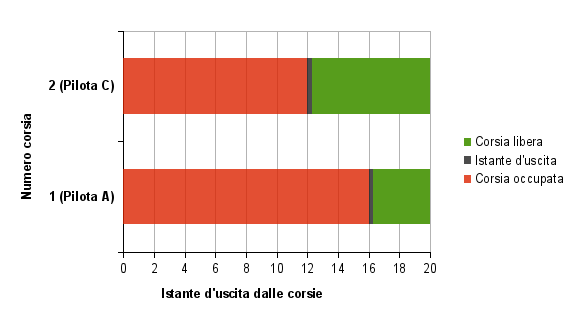
\includegraphics[width=110mm,bb=0 0 575 338]{./Immagini/AccessoSegmentiCaso2.png}}
	    % AccessoSegmentiStatoInziale.png: 575x338 pixel, 72dpi, 20.28x11.92 cm, bb=0 0 575 338
	    \caption{Caso 2: Stato del segmento S dopo che il pilota C ha effettuato l'accesso}
	    \label{fgr:AccessoSegmentiCaso2}
	  \end{figure}
	
	\subsubsection{Caso $T_i > T_b$}
	  In questo caso il pilota $P_c$ uscirebbe sia dopo $P_a$ che dopo $P_c$, per lui il segmento
	  è virtualmente libero in quanto nessuno dei 2 piloti gli crea intralcio. $P_c$ attraverserà
	  dunque il segmento in tempo $T_r = T_i$ utilizzando comunque la corsia con il tempo d'uscita monore,
	  ovvero $C_2$.
	  
	  Lo stato della risorsa protetta associata al segmento $S$ sarà modificata ponendo $T_C2 = T_r$,
	  come rappresentato in figura \ref{fgr:AccessoSegmentiCaso3}, e l'ordine d'uscita sarà come previsto
	  $P_a -> P_b -> P_c$.
	
	  \begin{figure}[h]
	    \centering
	    \fbox{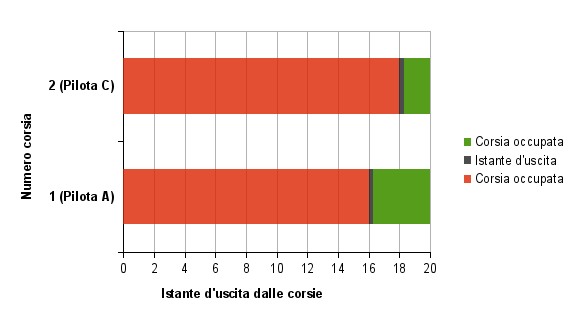
\includegraphics[width=110mm,bb=0 0 575 338]{./Immagini/AccessoSegmentiCaso3.png}}
	    % AccessoSegmentiStatoInziale.png: 575x338 pixel, 72dpi, 20.28x11.92 cm, bb=0 0 575 338
	    \caption{Caso 3: Stato del segmento S dopo che il pilota C ha effettuato l'accesso}
	    \label{fgr:AccessoSegmentiCaso3}
	  \end{figure}
	  
    \section{Distribuzione}
	% \<TO DO\>
	
  \chapter{Implementazione}
    Dato che il progetto presenta alcune problematiche di concorrenza, per la sua realizzazione è stato scelto
    di utilizzare il linguaggio di programmazione ADA.
    
    Di seguito verrà descritto come sono state realizzate le varie entità
    
    \section{Circuito}
  
  \chapter{Configurazione}
      
  
  \chapter{Compilazione ed esecuzione}

\end{document}
